\subsection[STL]{The STL}

\begin{frame}[fragile]
  \frametitlecpp[98]{The Standard Template Library}
  \begin{block}{What it is}
    \begin{itemize}
    \item A library of standard templates
    \item Has almost everything you need
      \begin{itemize}
      \item strings, containers, iterators
      \item algorithms, functions, sorters
      \item functors, allocators
      \item ...
      \end{itemize}
    \item Portable
    \item Reusable
    \item Efficient
    \end{itemize}
  \end{block}
  \pause
  \begin{exampleblock}{Use it}
    and adapt it to your needs, thanks to templates
  \end{exampleblock}
\end{frame}

\begin{frame}[fragile,label=STLcode]
  \frametitlecpp[14]{STL in practice}
  \begin{cppcode*}{}
    #include <vector>
    #include <algorithm>

    std::vector<int> vi{5, 3, 4}; // initializer list
    std::vector<int> vr(3); // constructor taking int

    std::transform(vi.begin(), vi.end(),      // range1
                   vi.begin(),          // start range2
                   vr.begin(),          // start result
                   std::multiplies{}); // function objects

    for(auto n : vr) {
      std::cout << n << ' ';
    }
  \end{cppcode*}
\end{frame}

\begin{frame}[fragile]
  \frametitlecpp[98]{STL's concepts}
  \begin{block}{containers}
    \begin{itemize}
    \item data structures for managing a range of elements
    \item irrespective of
      \begin{itemize}
      \item the data itself (templated)
      \item the memory allocation of the structure (templated)
      \item the algorithms that may use the structure
      \end{itemize}
    \item examples
      \begin{itemize}
      \item string, string\_view (\cpp17)
      \item list, forward\_list (\cpp11), vector, deque, array (\cpp11)
      \item map, set, multimap, multiset
      \item unordered\_map (\cpp11), unordered\_set (\cpp11)
      \item stack, queue, priority\_queue
      \item span (\cpp20)
      \end{itemize}
    \item non-containers: pair, tuple (\cpp11), optional (\cpp17), variant (\cpp17), any (\cpp17)
    \item see also the \href{https://en.cppreference.com/w/cpp/string/basic_string}{string} and \href{https://en.cppreference.com/w/cpp/container}{container library} on cppreference
    \end{itemize}
  \end{block}
\end{frame}

\begin{frame}[fragile]
  \frametitlecpp[11]{Containers: std::vector}
  \begin{cppcode*}{}
    #include <vector>
    std::vector<T> v{5, 3, 4}; // 3 Ts, 5, 3, 4
    std::vector<T> v(100);     // 100 default constr. Ts
    std::vector<T> v(100, 42); // 100 Ts with value 42
    std::vector<T> v2 = v;            // copy
    std::vector<T> v2 = std::move(v); // move, v is empty

    std::size_t s = v.size();
    bool empty = v.empty();

    v[2] = 17;         // write element 2
    T& t = v[1000];    // access element 1000, bug!
    T& t = v.at(1000); // throws std::out_of_range
    T& f = v.front();  // access first element
    v.back() = 0;     // write to last element
    T* v.data();       // pointer to underlying storage
  \end{cppcode*}
\end{frame}

\begin{frame}[fragile]
  \frametitlecpp[11]{Containers: std::vector}
  \begin{cppcode*}{}
    std::vector<T> v = ...;
    auto b = v.begin(); // iterator to first element
    auto e = v.end();   // iterator to one past last element
    // all following operations, except reserve, invalidate
    // all iterators (b and e) and references to elements

    v.resize(100); // size changes, grows: new T{}s appended
                   //           shrinks: Ts at end destroyed
    v.reserve(1000); // size remains, memory increased
    for (T i = 0; i < 900; i++)
      v.push_back(i); // add to the end
    v.insert(v.begin()+3, T{}); // insert after 3rd position

    v.pop_back();         // removes last element
    v.erase(v.end() - 3); // removes 3rd-last element
    v.clear();            // removes all elements
  \end{cppcode*}
\end{frame}

\begin{frame}[fragile]
  \frametitlecpp[98]{STL's concepts}
  \begin{block}{iterators}
    \begin{itemize}
    \item generalization of pointers
    \item allow iteration over some data
    \item irrespective of
      \begin{itemize}
      \item the container used (templated)
      \item the data itself (container is templated)
      \item the consumer of the data (templated algorithm)
      \end{itemize}
    \item examples
      \begin{itemize}
      \item iterator
      \item reverse\_iterator
      \item const\_iterator
      \end{itemize}
    \end{itemize}
  \end{block}
\end{frame}

\begin{frame}[fragile]
  \frametitlecpp[98]{STL's concepts}
  \begin{block}{algorithms}
    \begin{itemize}
    \item implementation of an algorithm working on data
    \item with a well defined behavior (defined complexity)
    \item irrespective of
      \begin{itemize}
      \item the data handled
      \item the container where the data live
      \item the iterator used to go through data (almost)
      \end{itemize}
    \item examples
      \begin{itemize}
      \item for\_each, find, find\_if, count, count\_if, search
      \item copy, swap, transform, replace, fill, generate
      \item remove, remove\_if
      \item unique, reverse, rotate, shuffle, partition
      \item sort, partial\_sort, merge, make\_heap, min, max
      \item lexicographical\_compare, iota, reduce, partial\_sum
      \end{itemize}
    \item see also \href{https://www.youtube.com/watch?v=2olsGf6JIkU}{105 STL Algorithms in Less Than an Hour} and the \href{https://en.cppreference.com/w/cpp/algorithm}{algorithms library} on cppreference
    \end{itemize}
  \end{block}
\end{frame}

\begin{frame}[fragile]
  \frametitlecpp[98]{STL's concepts}
  \begin{block}{functors / function objects}
    \begin{itemize}
      \item generic utility functions
      \item as structs with \mintinline{cpp}{operator()}
      \item mostly useful to be passed to STL algorithms
    \item implemented independently of
      \begin{itemize}
      \item the data handled (templated)
      \item the context (algorithm) calling it
      \end{itemize}
    \item examples
      \begin{itemize}
      \item plus, minus, multiplies, divides, modulus, negate
      \item equal\_to, less, greater, less\_equal, ...
      \item logical\_and, logical\_or, logical\_not
      \item bit\_and, bit\_or, bit\_xor, bit\_not
      \item identity, not\_fn
      \item bind, bind\_front
      \end{itemize}
    \item see also documentation on \href{https://en.cppreference.com/w/cpp/utility/functional}{cppreference}
    \end{itemize}
  \end{block}
\end{frame}

\begin{frame}[fragile]
  \frametitlecpp[11]{Functors / function objects}
  \begin{block}{Example}
    \begin{cppcode*}{}
      struct Incrementer {
        int m_inc;
        Incrementer(int inc) : m_inc(inc) {}

        int operator()(int value) const {
          return value + m_inc;
        }
      };
      std::vector<int> v;
      v.push_back(5); v.push_back(3); ...
      std::transform(v.begin(), v.end(), v.begin(),
                     Incrementer{42});
      \end{cppcode*}
    \end{block}
\end{frame}

\againframe{STLcode}

\begin{frame}[fragile]
  \frametitlecpp[11]{Range-based for loops with STL containers}
  \begin{block}{Iterator-based loop (since \cpp98)}
    \begin{cppcode*}{}
      std::vector<int> v = ...;
      int sum = 0;
      for (std::vector<int>::iterator it = v.begin();
           it != v.end(); it++)
        sum += *it;
    \end{cppcode*}
  \end{block}
  \pause
  \begin{block}{Range-based for loop (since \cpp11)}
    \begin{cppcode*}{firstnumber=6}
      std::vector<int> v = ...;
      int sum = 0;
      for (auto a : v) { sum += a; }
    \end{cppcode*}
  \end{block}
  \pause
  \begin{exampleblock}{STL way (since \cpp98)}
    \begin{cppcode*}{firstnumber=9}
      std::vector<int> v = ...;
      int sum = std::accumulate(v.begin(), v.end(), 0);
      // std::reduce(v.begin(), v.end(), 0); // C++17
    \end{cppcode*}
  \end{exampleblock}
\end{frame}

\begin{frame}[fragile]
  \frametitlecpp[98]{STL and functors}
  \begin{cppcode}
    // Finds the first element in a list between 1 and 10.
    list<int> l = ...;
    ...
    list<int>::iterator it =
      find_if(l.begin(), l.end(),
              compose2(logical_and<bool>(),
                       bind2nd(greater_equal<int>(), 1),
                       bind2nd(less_equal<int>(), 10)));

    // Computes sin(x)/(x + DBL_MIN) for elements of a range.
    transform(first, last, first,
              compose2(divides<double>(), // non-standard
                       ptr_fun(sin),
                       bind2nd(plus<double>(), DBL_MIN)));
  \end{cppcode}
  \begin{alertblock}{Deprecation warning}
  	Binders and function adaptors were removed in \cpp17 or \cpp20
  \end{alertblock}
\end{frame}

\begin{frame}[fragile]
  \frametitlecpp[14]{STL and lambdas}
  \begin{cppcode}
    // Finds the first element in a list between 1 and 10.
    std::list<int> l = ...;
    ...
    const auto it =
      std::find_if(l.begin(), l.end(),
        [](int i) { return i >= 1 && i <= 10; });

    // Computes sin(x)/(x + DBL_MIN) for elements of a range.
    std::transform(first, last, first,
      [](auto x) { return sin(x)/(x + DBL_MIN); });
  \end{cppcode}
\end{frame}

\begin{frame}[fragile]
  \frametitlecpp[98]{Welcome to lego programming!}
  \begin{block}{}
    \pgfdeclareimage[height=0.5cm]{AtlasLego}{morelanguage/AtlasLego.jpg}
    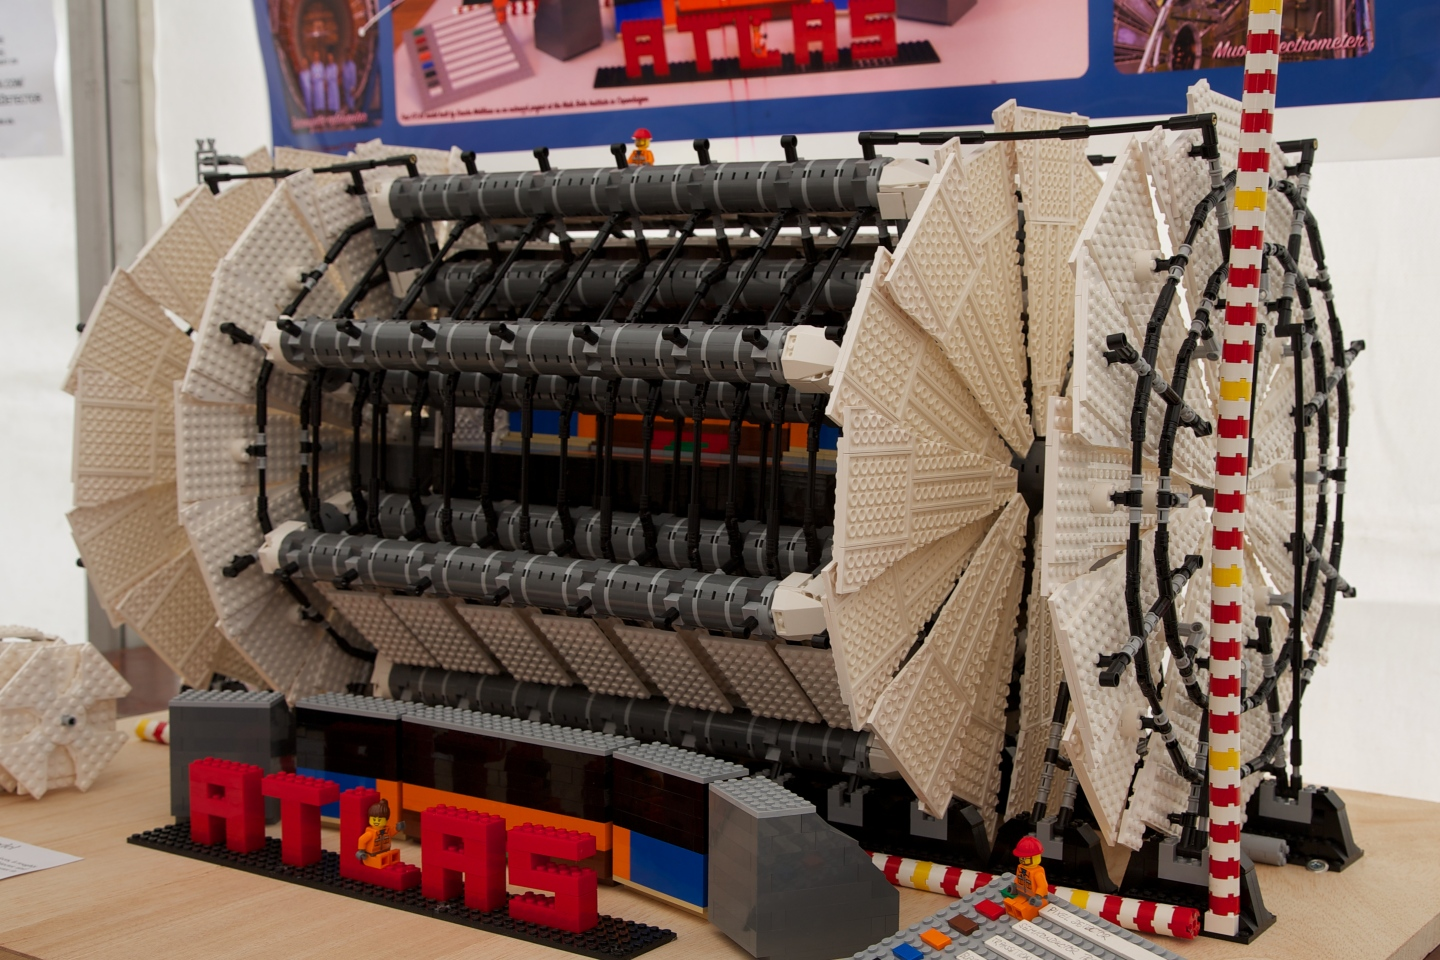
\includegraphics[width=\linewidth]{morelanguage/AtlasLego}
  \end{block}
\end{frame}

\begin{frame}[fragile]
  \frametitlecpp[98]{Using the STL}
  \begin{alertblock}{Exercise Time}
    \begin{itemize}
    \item go to code/stl
    \item look at the non STL code in randomize.nostl.cpp
      \begin{itemize}
        \item it creates a vector of ints at regular intervals
        \item it randomizes them
        \item it computes differences between consecutive ints
        \item and the mean and variance of it
      \end{itemize}
    \item open randomize.cpp and complete the ``translation'' to STL
    \item see how easy it is to reuse the code with complex numbers
    \end{itemize}
  \end{alertblock}
\end{frame}

\begin{frame}[fragile]
  \frametitlecpp[98]{Using the STL}
  \begin{exampleblock}{Be brave and persistent!}
    \begin{itemize}
    \item you may find the STL quite difficult to use
    \item template syntax is really tough
    \item it is hard to get right, compilers spit out long error novels
    \begin{itemize}
      \item but, compilers are getting better with error messages
    \end{itemize}
    \item \cpp20 will help with concepts and ranges
    \item the STL is extremely powerful and flexible
    \item it will be worth your time!
    \end{itemize}
  \end{exampleblock}
\end{frame}
